\documentclass[14 pt]{extarticle}

	\usepackage[frenchb]{babel}
	\usepackage[utf8]{inputenc}  
	\usepackage[T1]{fontenc}
	\usepackage{amssymb}
	\usepackage[mathscr]{euscript}
	\usepackage{stmaryrd}
	\usepackage{amsmath}
	\usepackage{tikz}
	\usepackage[all,cmtip]{xy}
	\usepackage{amsthm}
	\usepackage{varioref}
	\usepackage{geometry}
	\geometry{a4paper}
	\usepackage{lmodern}
	\usepackage{hyperref}
	\usepackage{array}
	 \usepackage{fancyhdr}
	 \usepackage{float}
\renewcommand{\theenumi}{\alph{enumi})}
	\pagestyle{fancy}
	\theoremstyle{plain} 
	\fancyfoot[C]{} 
	\fancyhead[L]{}
	\fancyhead[R]{}\geometry{
 a4paper,
 total={170mm,257mm},
 left=10mm,
 top=15mm,
 bottom = 10mm
 }
	
	
	\title{Contrôle début de second trimestre}
	\date{}
	\begin{document}
	{\begin{center}{\Large{Contrôle début de second trimestre}}\end{center}}
\subsection*{Exercice 1 - 6 points}	%(1 + 2 + 2 + 1) 
Calculez le volume des figures suivantes, en centimètres cube. \begin{enumerate}
\item Un cube d'arête $4$ cm. 
\item Un pavé droit de largeur $3$ mm, de longueur $5$ dm et de hauteur $2$ mm. 
\item Un cône de rayon $3$ cm et de hauteur $4$ cm. (Donnez la formule exacte, puis la valeur approchée à l'unité en $\mathrm{cm}^3$.)
\item Une pyramide de hauteur $3$ cm et dont la base est un carré de côté $2$ cm. 

\end{enumerate}

\subsection*{Exercice 2 (4 points)} % 1+ 1 + 2
 Développer et réduire les expressions suivantes :\begin{enumerate}
 \item $ (x+1) - (x+2)$
 \item $5 \times (x+3) $
 \item $(x+1) \times 2 - 4\times (x-1)$. 
\end{enumerate}    

\ \ \ 


\ \ \ 


\ \ \ 

\textbf{Suite au dos de la feuille}
  
  
  \subsection*{Exercice 3 (10 points)}

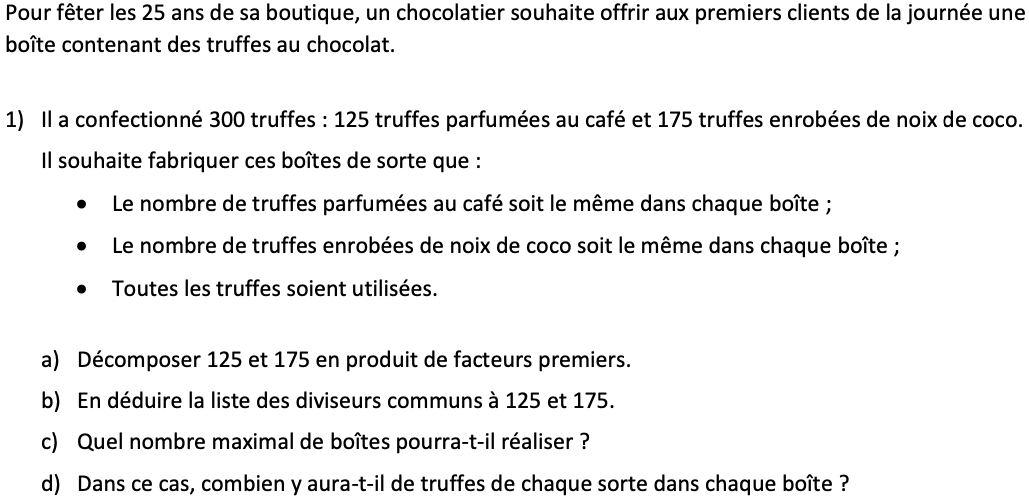
\includegraphics[scale=1]{Brevet.png} 
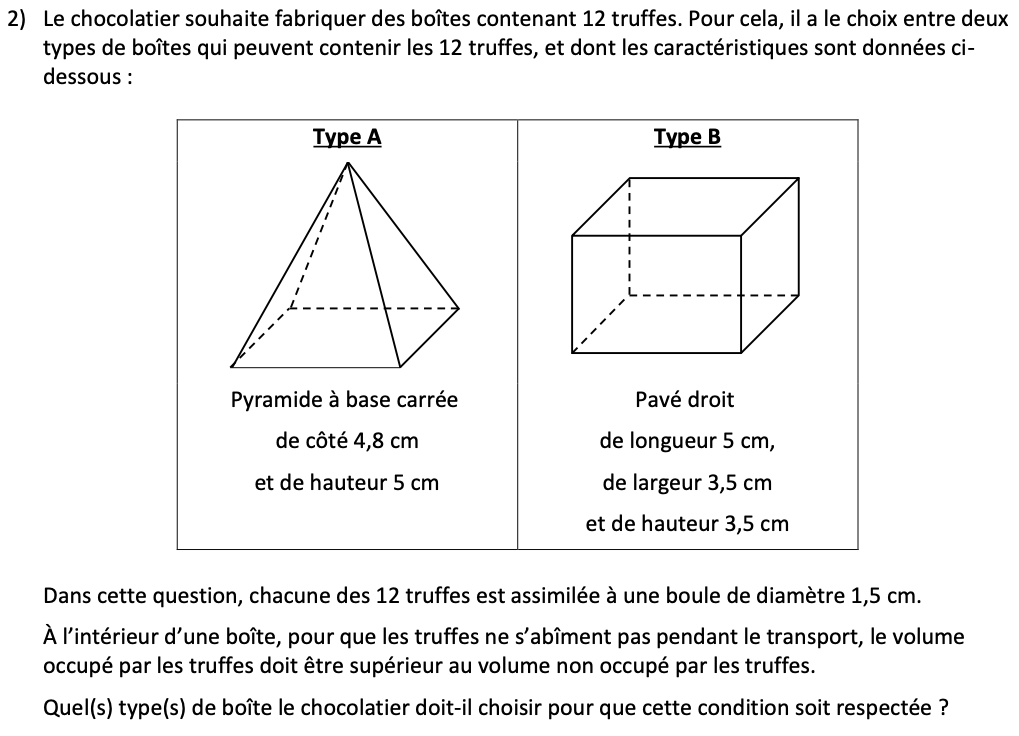
\includegraphics[scale=1]{Brevet2.png} 
 
 \newpage
 
	{\begin{center}{\Large{Contrôle début de second trimestre}}\end{center}}
	
\subsection*{Exercice 1 - 6 points}	%(1 + 2 + 2 + 1) 
Calculez le volume des figures suivantes, en centimètres cube. \begin{enumerate}
\item Un cube d'arête $4$ cm. 
\item Un pavé droit de largeur $3$ mm, de longueur $5$ dm et de hauteur $2$ mm. 
\item Un cône de rayon $3$ cm et de hauteur $4$ cm. (Donnez la formule exacte, puis la valeur approchée à l'unité en $\mathrm{cm}^3$.)
\item Une pyramide de hauteur $3$ cm et dont la base est un carré de côté $2$ cm. 

\end{enumerate}

\subsection*{Exercice 2 (4 points)} % 1+ 1 + 2
 Développer et réduire les expressions suivantes :\begin{enumerate}
 \item $ (y+5) - (y+2)$
 \item $6 \times (y-1) $
 \item $(y+2) \times 2 - 3\times (y-1)$. 
\end{enumerate}    

\ \ \ 


\ \ \ 


\ \ \ 

\textbf{Suite au dos de la feuille}
  
  \subsection*{Exercice 3 (10 points)}

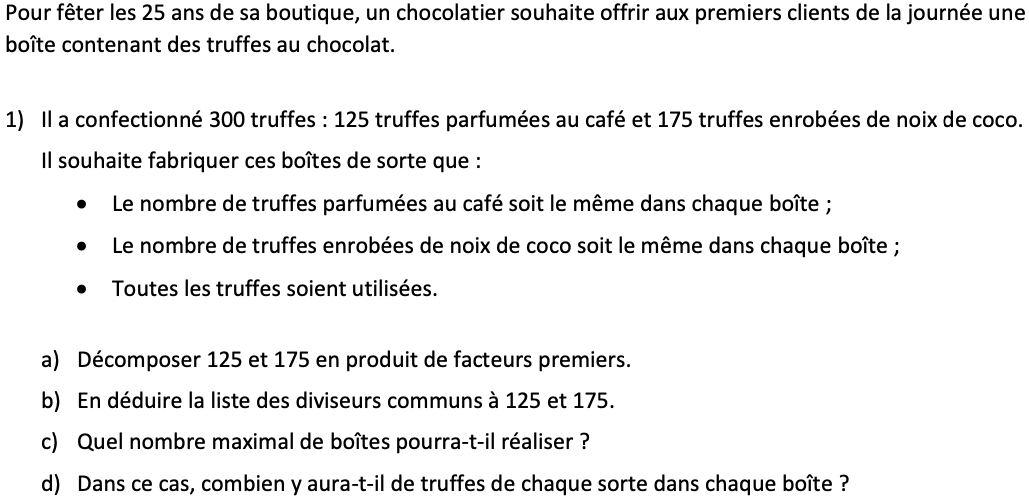
\includegraphics[scale=1]{Brevet.png} 
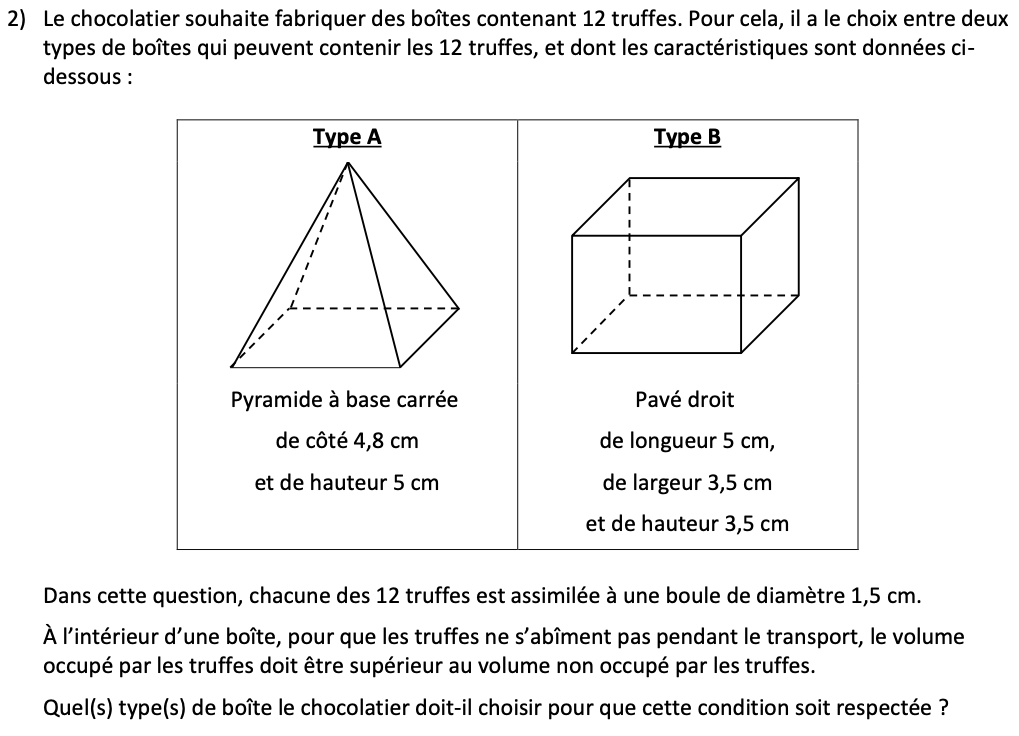
\includegraphics[scale=1]{Brevet2.png} 
 	\end{document}
